\documentclass[a4paper,12pt]{article}
\usepackage{cmap}
\usepackage[cp1251]{inputenc}
\usepackage[english, ukrainian, russian]{babel}
\usepackage[left=2cm,right=1.5cm,top=1cm,bottom=1cm]{geometry}
\usepackage{amssymb}
\usepackage{graphicx}

\begin{document}

\pagenumbering{gobble}


\begin{large}

\begin{center}
\section*{Deep Learning}
\end{center}



\medskip
\medskip

\hrule height 1pt
\vskip 3pt \hrule

\medskip
\medskip
\medskip

\textbf{AlexNet}

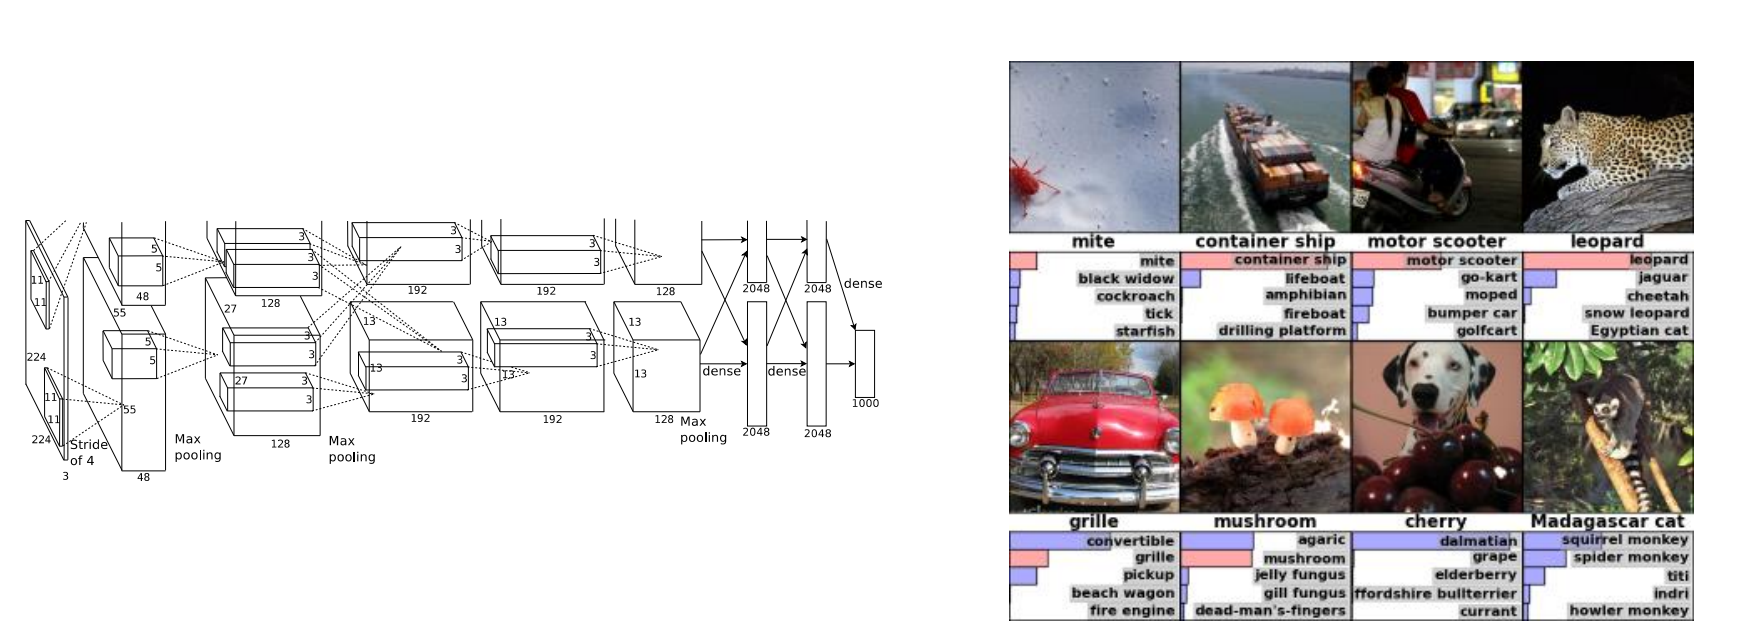
\includegraphics[scale=0.4]{dl1}

�AlexNet� (Krizhevsky et al., 2012), winning entry of ImageNet 2012 competition
with a Top-5 error rate of 15.3\% (next best system with highly engineered features
based got 26.1\% error) 

\medskip
\medskip

\textbf{AlphaGo}

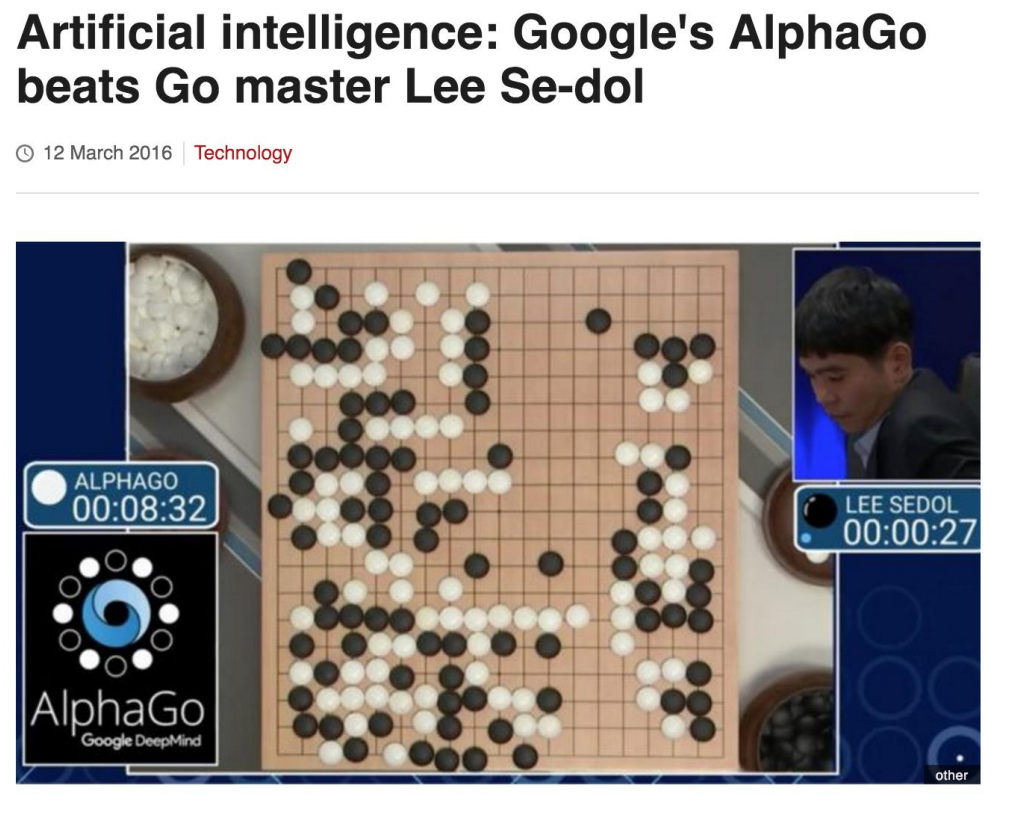
\includegraphics[scale=0.6]{dl2}

\medskip
\medskip

\textbf{Neural networks for machine learning}

The term �neural network� largely refers to the hypothesis class part of a machine
learning algorithm:

1. Hypothesis: non-linear hypothesis function, which involve compositions of
multiple linear operators (e.g. matrix multiplications) and elementwise nonlinear functions

2. Loss: �Typical� loss functions for classification and regression: logistic, softmax
(multiclass logistic), hinge, squared error, absolute error

3. Optimization: Gradient descent, or more specifically, a variant called
stochastic gradient descent we will discuss shortly

\medskip
\medskip

\textbf{Linear hypotheses and feature learning}

Until now, we have (mostly) considered machine learning algorithms that linear
hypothesis class

$$h_{\theta}(x)=\theta^{T}\phi(x)$$

where $\phi:\mathbb{R}^{n}\rightarrow\mathbb{R}^{k}$ denotes some set of typically non-linear features

Example: polynomials, radial basis functions, custom features like TFIDF (in many
domains every 10 years or so there would be new feature types)

The performance of these algorithms depends crucially on coming up with good
features

Key question: can we come up with an algorithm that will automatically learn the
features themselves?

Instead of a simple linear classifier, let�s consider a two-stage hypothesis class
where one linear function creates the features and another produces the final
hypothesis

$$h_{\theta}(x) = W_{2}\phi(x) +b_{2} = W_{2}(W_{1}x+ b_{1}) + b_{2},$$

$$\theta = \{W_{1}\in \mathbb{R}^{k\times n}, b_{1}\in \mathbb{R}^{k}, W_{2}\in \mathbb{R}^{1\times k}, b_{2}\in \mathbb{R}\}$$

But there is a problem:

$$h_{\theta}(x) =  W_{2}(W_{1}x+ b_{1}) + b_{2} = \tilde{W}x + \tilde{b}$$

i.e., we are still just using a linear classifier (the apparent added complexity is
actually not changing the underlying hypothesis function)




\end{large}
\end{document}

